\documentclass[
  aspectratio=169,
]{beamer}

\usepackage[slovak]{babel}
\usepackage{svg}
\usepackage{listings}
\usepackage[utf8]{inputenc}
\usepackage[T1]{fontenc}
\usepackage{csquotes}
\usepackage{expl3,biblatex}
\addbibresource{example.bib}
\usepackage{booktabs}
\usetheme[
  workplace=fi,
  locale=czech,
]{MU}

\usepackage{listings}
\usepackage{color}

\definecolor{mygreen}{rgb}{0,0.6,0}
\definecolor{mygray}{rgb}{0.5,0.5,0.5}
\definecolor{mymauve}{rgb}{0.58,0,0.82}

\lstset{
  basicstyle=\footnotesize,
  breakatwhitespace=false,
  breaklines=true,
  captionpos=b,
  commentstyle=\color{mygreen},
  deletekeywords={...},
  escapeinside={\%*}{*)},
  extendedchars=true,
  firstnumber=1000,
  frame=none,
  keepspaces=true,
  keywordstyle=\color{blue},
  language=Python,
  morekeywords={*,...},
  numbers=none,
  numbersep=5pt,
  numberstyle=\tiny\color{mygray},
  rulecolor=\color{black},
  showspaces=false,
  showstringspaces=false,
  showtabs=false,
  stepnumber=2,
  stringstyle=\color{mymauve},
  tabsize=4,
  title=\lstname,
}

\title[Structure Quality Control]{Replikácia funkcionality PDB validačného servera v prostredí MetaCentra}
\subtitle[Alternatívny názov prezentácie]{Structure Quality Control}
\author[M.\, Jediný]{Martin Jediný\texorpdfstring{\\}{, }514269@mail.muni.cz}
\institute[FI MU]{Fakulta informatiky Masarykovej univerzity}
\date{\today}
\subject{Predmet prezentace}
\keywords{kľúčové, slová, prezentácie}
\begin{document}


\begin{frame}[plain]
\maketitle
\end{frame}

\begin{frame}{Biomakromolekuly}
\begin{itemize}
  \item Hrajú kľúčovú úlohu v rôznych biologických procesoch
  \item Veľmi veľké molekuly --- tisíce a viac opakujúcich sa jednotiek
  \begin{itemize}
    \item Bielkoviny
    \item Nukleové kyseliny
    \item Polysacharidy
  \end{itemize}
  \item Funkcia určená štruktúrou
  \item Určenie štruktúry je nevyhnutné pre pochopenie biologických procesov
\end{itemize}
\end{frame}

\begin{frame}{Štrukturálne dáta}
\begin{itemize}
  \item Polohy atómov v trojrozmernom priestore
  \item Determinované pomocou rôznych experimentálnych metód
  \begin{itemize}
    \item Potenciál na vznik chýb
  \end{itemize}
  \item Nutná validácia výsledných dát
\end{itemize}
\end{frame}

\begin{frame}{Structure Quality Control}
\begin{itemize}
  \item Protein Data Bank (PDB) poskytuje verejný validačný server 
  \item Nedostatočný na niektoré výskumné projekty SB-NCBR\footnote{Structural bioinformatics research group at National Centre for Biomolecular Research}
  \begin{itemize}
    \item Validácie miliónov malých štruktúr (e.g.\ \emph{AlphaFoldDB})
    \item Rýchla iteratívna validácia pre optimizáciu štruktúr
  \end{itemize}
  \item Implementujeme službu Structure Quality Control (SQC), ktorá spĺňa požiadavky SB-NCBR
\end{itemize}
\end{frame}

\begin{frame}{Structure Quality Control}
\begin{itemize}
  \item Služba využíva existujúce nástroje na validáciu štruktúr
  \item Nástroje sú integrové do služby s jediným prístupovým bodom
  \item Škálovateľnosť je dôležitou vlastnosťou implementácie
  \item Hlavná inštancia je nasadená v Kubernetes clusteri poskytnutom virtuálnou organizáciou MetaCentrum
  \item Implementované rozhrania v Python a Bash
\end{itemize}
\end{frame}

\begin{frame}{Návrh}
\begin{figure}
  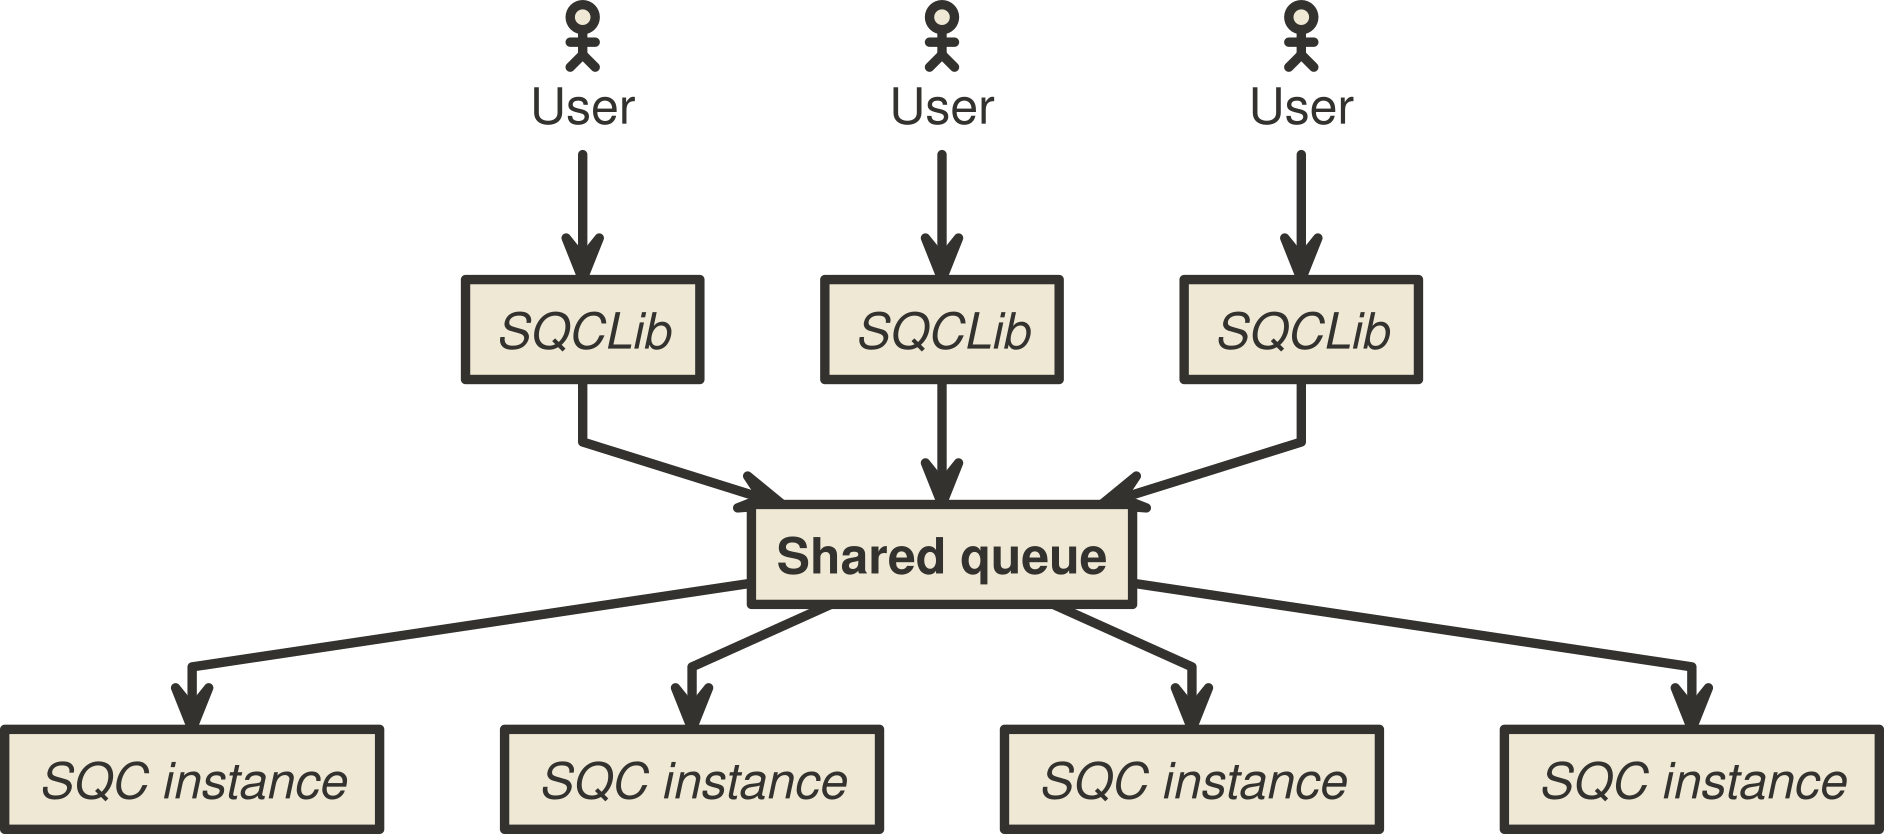
\includegraphics[width=.8\textwidth,height=.8\textheight,keepaspectratio]{img/diagram.png}
  % \caption{Zdieľaná fronta je implementovaná pomocou služby na posielanie správ RabbitMQ. Škálovanie automaticky rieši Kubernetes.}
\end{figure}
\end{frame}

\begin{frame}{Implementácia}
\begin{itemize}
  \item Docker využitý na zjednodušenie nasadenia
  \item Ako úložisko je použitá služba MinIO
  \begin{itemize}
    \item Open-source alternatíva k Amazon S3 s rovnakým API
  \end{itemize}
  \item Kombinácia služby na posielanie správ RabbitMQ a úložiska MinIO
        implementuje vzor Producent-Konzument
  \item Všetky služby nasadené pomocou Kubernetes
  \begin{itemize}
    \item Implementácia škálovania
  \end{itemize}
\end{itemize}
\end{frame}

\begin{frame}{Škálovanie replík}
\begin{figure}
  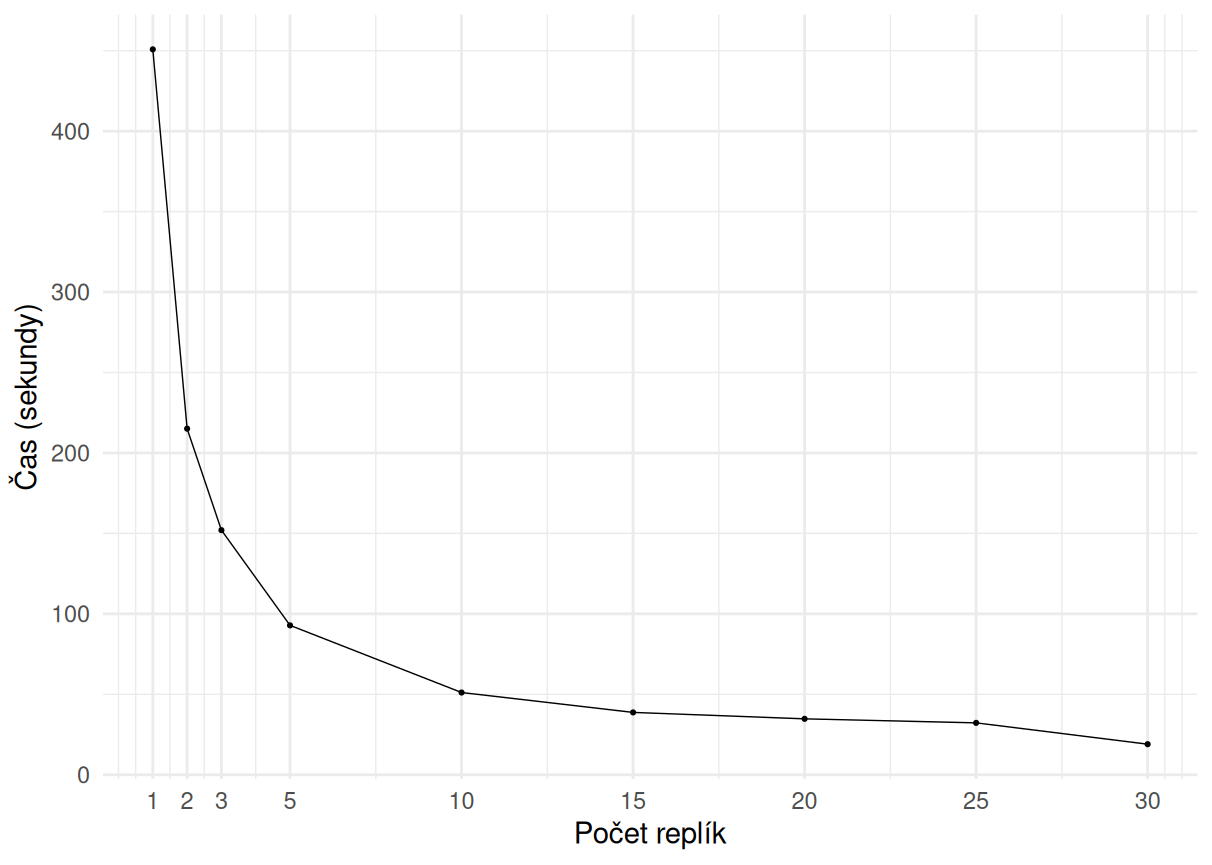
\includegraphics[width=.8\textwidth,height=.8\textheight,keepaspectratio]{img/replica-perf.png}
  \caption{Graf znázorňujúci dopad škálovania SQC inštancií na rýchlosť validácie tridsiatich štruktúr.}
\end{figure}
\end{frame}

\begin{frame}{Výsledky práce}
\begin{itemize}
  \item Implementácia horizontálne škáľovateľnej validačnej služby
  \begin{itemize}
    \item integruje validačné nastroje vyvinuté komunitou
    \item jasne definované výstupy služby
  \end{itemize}

  \item Implementácia jednoduchých programovacích rozhraní k službe
  \begin{itemize}
    \item v jazykoch Python a Bash
  \end{itemize}

  \item Nasadenie do Kubernetes prostredí je automatizované pomocou Ansible
  \item Inštancia služby je nasadená v prostredí MetaCentra a je pripravená na použitie v projektoch SB-NCBR
\end{itemize}
\end{frame}

\end{document}
